%
% This is the LaTeX template file for lecture notes for EE 382C/EE 361C.
%
% To familiarize yourself with this template, the body contains
% some examples of its use.  Look them over.  Then you can
% run LaTeX on this file.  After you have LaTeXed this file then
% you can look over the result either by printing it out with
% dvips or using xdvi.
%
% This template is based on the template for Prof. Sinclair's CS 270.


\documentclass[twoside]{article}
\usepackage{graphicx}
\setlength{\oddsidemargin}{0.25 in}
\setlength{\evensidemargin}{-0.25 in}
\setlength{\topmargin}{-0.6 in}
\setlength{\textwidth}{6.5 in}
\setlength{\textheight}{8.5 in}
\setlength{\headsep}{0.75 in}
\setlength{\parindent}{0.25 in}
\setlength{\parskip}{0.1 in}
\usepackage{graphics}
\usepackage{algorithm}
\usepackage{mathtools}
\usepackage{mathptmx}
\usepackage{algpseudocode}
\usepackage{caption}
\usepackage{listings}
\newcommand{\forceindent}{\leavevmode{\parindent=2em\indent}}
\newcounter{magicrownumbers}
\newcommand\rownumber{\stepcounter{magicrownumbers}\arabic{magicrownumbers}}
\usepackage[colorlinks]{hyperref}

%
% The following commands set up the lecnum (lecture number)
% counter and make various numbering schemes work relative
% to the lecture number.
%
\newcounter{lecnum}
\renewcommand{\thepage}{\thelecnum-\arabic{page}}
\renewcommand{\thesection}{\thelecnum.\arabic{section}}
\renewcommand{\theequation}{\thelecnum.\arabic{equation}}
\renewcommand{\thefigure}{\thelecnum.\arabic{figure}}
\renewcommand{\thetable}{\thelecnum.\arabic{table}}



%
% The following macro is used to generate the header.
%
\newcommand{\lecture}[4]{
   \pagestyle{myheadings}
   \thispagestyle{plain}
   \newpage
   \setcounter{lecnum}{#1}
   \setcounter{page}{1}
   \noindent
   \begin{center}
   \framebox{
      \vbox{\vspace{2mm}
    \hbox to 6.28in { {\bf EE 382C/361C: Multicore Computing
                        \hfill Fall 2016} }
       \vspace{4mm}
       \hbox to 6.28in { {\Large \hfill Lecture #1: #2  \hfill} }
       \vspace{2mm}
       \hbox to 6.28in { {\it Lecturer: #3 \hfill Scribe: #4} }
      \vspace{2mm}}
   }
   \end{center}
   \markboth{Lecture #1: #2}{Lecture #1: #2}
   %{\bf Disclaimer}: {\it These notes have not been subjected to the
   %usual scrutiny reserved for formal publications.  They may be distributed
   %outside this class only with the permission of the Instructor.}
   \vspace*{4mm}
}

%
% Convention for citations is authors' initials followed by the year.
% For example, to cite a paper by Leighton and Maggs you would type
% \cite{LM89}, and to cite a paper by Strassen you would type \cite{S69}.
% (To avoid bibliography problems, for now we redefine the \cite command.)
% Also commands that create a suitable format for the reference list.
\renewcommand{\cite}[1]{[#1]}
\def\beginrefs{\begin{list}%
        {[\arabic{equation}]}{\usecounter{equation}
         \setlength{\leftmargin}{2.0truecm}\setlength{\labelsep}{0.4truecm}%
         \setlength{\labelwidth}{1.6truecm}}}
\def\endrefs{\end{list}}
\def\bibentry#1{\item[\hbox{[#1]}]}

%Use this command for a figure; it puts a figure in wherever you want it.
%usage: \fig{NUMBER}{SPACE-IN-INCHES}{CAPTION}
\newcommand{\fig}[3]{
			\vspace{#2}
			\begin{center}
			Figure \thelecnum.#1:~#3
			\end{center}
	}
% Use these for theorems, lemmas, proofs, etc.
\newtheorem{theorem}{Theorem}[lecnum]
\newtheorem{lemma}[theorem]{Lemma}
\newtheorem{proposition}[theorem]{Proposition}
\newtheorem{claim}[theorem]{Claim}
\newtheorem{corollary}[theorem]{Corollary}
\newtheorem{definition}[theorem]{Definition}
\newenvironment{proof}{{\bf Proof:}}{\hfill\rule{2mm}{2mm}}

% **** IF YOU WANT TO DEFINE ADDITIONAL MACROS FOR YOURSELF, PUT THEM HERE:

\begin{document}
%FILL IN THE RIGHT INFO.
%\lecture{**LECTURE-NUMBER**}{**DATE**}{**LECTURER**}{**SCRIBE**}
\lecture{17}{October 25}{Vijay Garg}{Xin Xu}
%\footnotetext{These notes are partially based on those of Nigel Mansell.}

% **** YOUR NOTES GO HERE:

% Some general latex examples and examples making use of the
% macros follow.
%**** IN GENERAL, BE BRIEF. LONG SCRIBE NOTES, NO MATTER HOW WELL WRITTEN,
%**** ARE NEVER READ BY ANYBODY.
\section{Introduction}
The topics covered in this lecture are:
\begin{enumerate}
	\item Merge Sort
	\item Wait-Free Synchronization
\end{enumerate}

\section{Merge Sort}
Decompose one task into multiple tasks:
\begin{figure}[!ht]
  \centering
   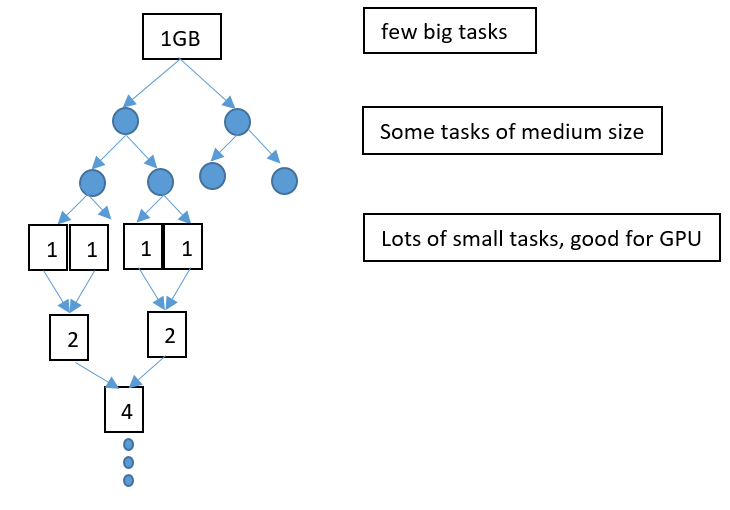
\includegraphics[height=0.35\textheight, width=0.72\textwidth]{./mergesort.png}
  \caption{Merge Sort}
    \label{model}
\end{figure}
\subsection{Algorithm for Multiple Merging tasks}
\begin{enumerate}
	\item Determine rank of each element(mentioned in Lecture9). Rank(x) is equal to the sum of number of elements in B less than x and the number of elements in C less than x. Then merge array B and array C to get array D.
	\item Cascaded Algorithm(mentioned in Lecture10). Divide n array into n/logn groups. Fill in only splitters.
   \begin{figure}[!ht]
  \centering
   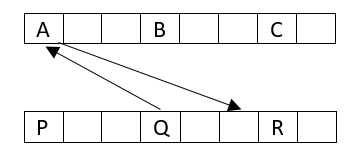
\includegraphics[height=0.1\textheight, width=0.3\textwidth]{./3.png}
  \caption{Merge Sort}
    \label{model}
\end{figure}
\end{enumerate}


\section{Wait-Free Synchronization}
It is possible to build a multiple � reader multiple writer(MRMW) atomic multivalued register from single-reader single-writer(SRSW) safe Boolean registers. This can be achieved by the following chain of constructions:
%Use this command for a figure; it puts a figure in wherever you want it.
%usage: \fig{NUMBER}{SPACE-IN-INCHES}{CAPTION}
\begin{figure}[!ht]
  \centering
   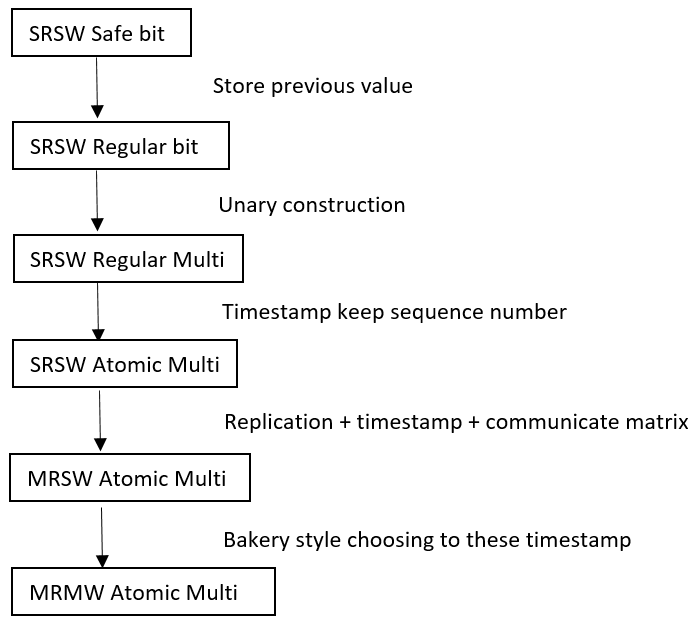
\includegraphics[height=0.35\textheight, width=0.72\textwidth]{./register.png}
  \caption{construction}
    \label{model}
\end{figure}
\subsection{Regular SRSW Register}
We construct a regular SRSW register from a safe SRSW register using smarter writer which can remember last value.
\begin{algorithm}
\caption{RegularBoolean}
\begin{algorithmic}[1]
\State class RegularBoolean \{
\State \indent    boolean prev; // not shared
\State \indent    SafeBoolean value;
\State \indent    public boolean getValue() \{
\State \indent \indent        return value.getValue();
\State \indent    \}
\State \indent     public void setValue(boolean b) \{
\State \indent \indent        if (prev != b) \{
\State \indent \indent \indent            value.setValue(b);
\State \indent \indent \indent            prev = b;
\State \indent \indent \}
\State \indent \}
\State \}
\end{algorithmic}
\label{alg:Regular SRSW}
\end{algorithm}
\subsection{SRSW Multivalued Register}
For read: scan the array, looking for the first non-zero bit. The idea is that the reader should return the index of the first true bit.
The straightforward solution for writer: Updating the array in the forward direction until it reaches the required index. But it does not work.\\
Reason: Suppose firstly we set A[3] to 1, and now we need to write A[5] to 1. After the writer executes, the array becomes  0 0 0 0. Before writer set A[5] to 1, the reader comes in, it will find all zeros.\\
For write, the right operation:\\
$\bullet$Set A[x] = 1\\
$\bullet$Traverse backward resetting bit to zeros\\
But it is not atomic. This situation can happen:
\begin{figure}[!ht]
  \centering
   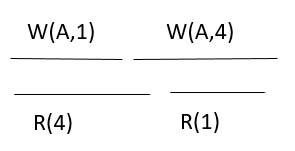
\includegraphics[height=0.1\textheight,width=0.3\linewidth] {./2.png}
    \label{model}
\end{figure}
\\
Code in the handout: the reader first does a forward scan and then does a backward scan at line 14
to find the first bit that is true. Two scans are sufficient to guarantee linearizability.\\

\subsection{MRSW Register}
We now build a MRSW register from SRSW registers. The straightforward solution is to have an array of n SRSW registers and one writer write to all n registers. This is not linearizable. Instead, we use a sequence number associated with each value.
The writer maintains the sequence number and writes this sequence number with any value that it writes.
Thus we view our SRSW register as consisting of two fields: the value and ts (for timestamp). In order to build MRSW Register, we use communication matrix. Comm[i][j] is used by the reader i to inform the value it read to the reader j. Reader communicate the value it read to all other readers by writing in the corresponding row.

\subsection{MRMW Register}
The construction of an MRMW register from MRSW registers is to use n MRSW registers for n writers. We use the approach of the Bakery algorithm to assign unique sequence number to each writer.
\subsection{Atomic Snapshots}
Lock-free constructions can be turned into wait-free constructions by using the notion of �helping� moves. The main idea is that a thread tries to help pending operations. For example, the thread wanting to perform an update operation helps another concurrent thread.

\section*{References}
\beginrefs
\bibentry{1}{\sc V.K.~Garg} Introduction to Multicore Computing
\bibentry{2} https://github.com/vijaygarg1/UT-Garg-EE382C-EE361C-Multicore
\endrefs


\end{document}





